\documentclass[10pt]{article}
\usepackage{tikz}
\usetikzlibrary{shapes.misc}
\usepackage[margin=0cm]{geometry}
\pagestyle{empty}
\tikzstyle{every node}=[cross out, draw, red]

\begin{document}

\vspace*{\fill}
\begin{center}
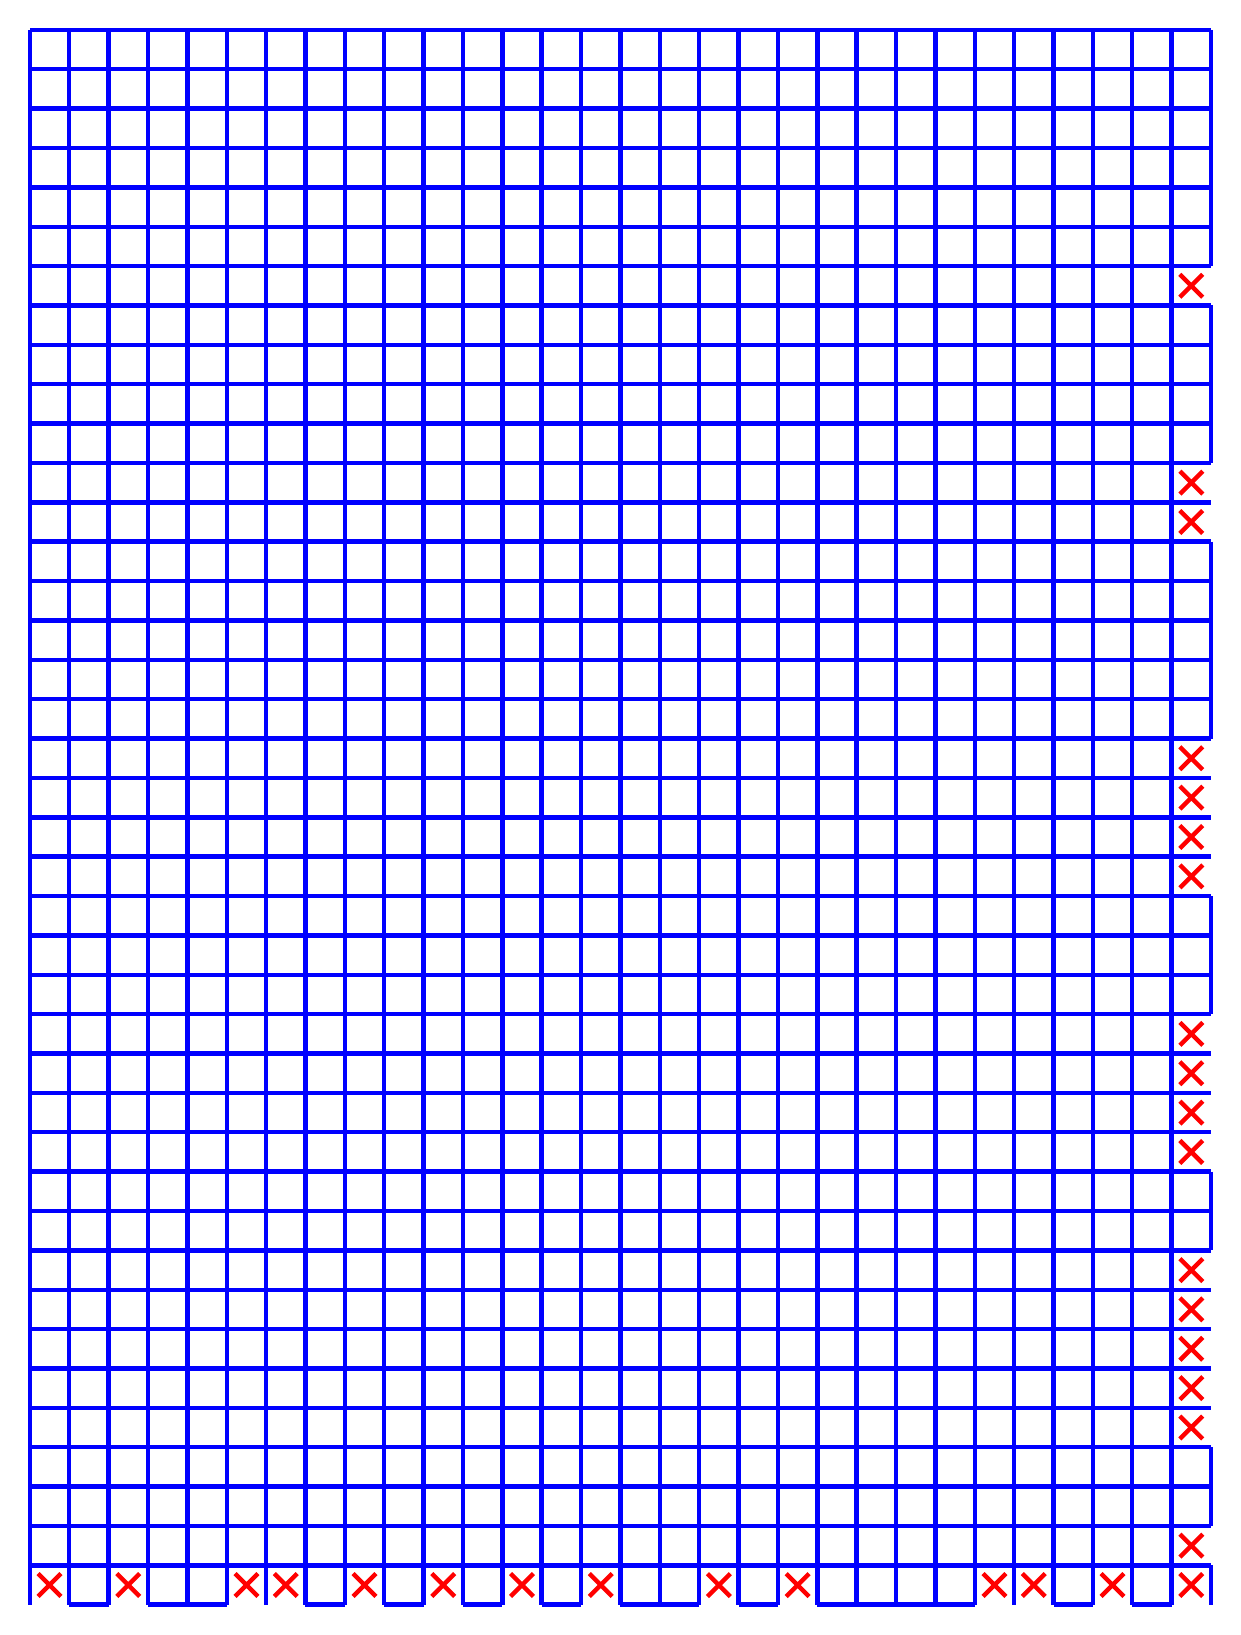
\begin{tikzpicture}[x=0.5cm, y=-0.5cm, ultra thick, blue]
% Walls
    \draw (0,0) -- (30,0);
    \draw (0,1) -- (30,1);
    \draw (0,2) -- (30,2);
    \draw (0,3) -- (30,3);
    \draw (0,4) -- (30,4);
    \draw (0,5) -- (30,5);
    \draw (0,6) -- (30,6);
    \draw (0,7) -- (30,7);
    \draw (0,8) -- (30,8);
    \draw (0,9) -- (30,9);
    \draw (0,10) -- (30,10);
    \draw (0,11) -- (30,11);
    \draw (0,12) -- (30,12);
    \draw (0,13) -- (30,13);
    \draw (0,14) -- (30,14);
    \draw (0,15) -- (30,15);
    \draw (0,16) -- (30,16);
    \draw (0,17) -- (30,17);
    \draw (0,18) -- (30,18);
    \draw (0,19) -- (30,19);
    \draw (0,20) -- (30,20);
    \draw (0,21) -- (30,21);
    \draw (0,22) -- (30,22);
    \draw (0,23) -- (30,23);
    \draw (0,24) -- (30,24);
    \draw (0,25) -- (30,25);
    \draw (0,26) -- (30,26);
    \draw (0,27) -- (30,27);
    \draw (0,28) -- (30,28);
    \draw (0,29) -- (30,29);
    \draw (0,30) -- (30,30);
    \draw (0,31) -- (30,31);
    \draw (0,32) -- (30,32);
    \draw (0,33) -- (30,33);
    \draw (0,34) -- (30,34);
    \draw (0,35) -- (30,35);
    \draw (0,36) -- (30,36);
    \draw (0,37) -- (30,37);
    \draw (0,38) -- (30,38);
    \draw (0,39) -- (30,39);
    \draw (1,40) -- (2,40);
    \draw (3,40) -- (5,40);
    \draw (7,40) -- (8,40);
    \draw (9,40) -- (10,40);
    \draw (11,40) -- (12,40);
    \draw (13,40) -- (14,40);
    \draw (15,40) -- (17,40);
    \draw (18,40) -- (19,40);
    \draw (20,40) -- (24,40);
    \draw (26,40) -- (27,40);
    \draw (28,40) -- (29,40);
    \draw (0,0) -- (0,40);
    \draw (1,0) -- (1,40);
    \draw (2,0) -- (2,40);
    \draw (3,0) -- (3,40);
    \draw (4,0) -- (4,40);
    \draw (5,0) -- (5,40);
    \draw (6,0) -- (6,40);
    \draw (7,0) -- (7,40);
    \draw (8,0) -- (8,40);
    \draw (9,0) -- (9,40);
    \draw (10,0) -- (10,40);
    \draw (11,0) -- (11,40);
    \draw (12,0) -- (12,40);
    \draw (13,0) -- (13,40);
    \draw (14,0) -- (14,40);
    \draw (15,0) -- (15,40);
    \draw (16,0) -- (16,40);
    \draw (17,0) -- (17,40);
    \draw (18,0) -- (18,40);
    \draw (19,0) -- (19,40);
    \draw (20,0) -- (20,40);
    \draw (21,0) -- (21,40);
    \draw (22,0) -- (22,40);
    \draw (23,0) -- (23,40);
    \draw (24,0) -- (24,40);
    \draw (25,0) -- (25,40);
    \draw (26,0) -- (26,40);
    \draw (27,0) -- (27,40);
    \draw (28,0) -- (28,40);
    \draw (29,0) -- (29,40);
    \draw (30,0) -- (30,6);
    \draw (30,7) -- (30,11);
    \draw (30,13) -- (30,18);
    \draw (30,22) -- (30,25);
    \draw (30,29) -- (30,31);
    \draw (30,36) -- (30,38);
    \draw (30,39) -- (30,40);
% Pillars
% Inner points in accessible cul-de-sacs
    \node at (29.5,6.5) {};
    \node at (29.5,11.5) {};
    \node at (29.5,12.5) {};
    \node at (29.5,18.5) {};
    \node at (29.5,19.5) {};
    \node at (29.5,20.5) {};
    \node at (29.5,21.5) {};
    \node at (29.5,25.5) {};
    \node at (29.5,26.5) {};
    \node at (29.5,27.5) {};
    \node at (29.5,28.5) {};
    \node at (29.5,31.5) {};
    \node at (29.5,32.5) {};
    \node at (29.5,33.5) {};
    \node at (29.5,34.5) {};
    \node at (29.5,35.5) {};
    \node at (29.5,38.5) {};
    \node at (0.5,39.5) {};
    \node at (2.5,39.5) {};
    \node at (5.5,39.5) {};
    \node at (6.5,39.5) {};
    \node at (8.5,39.5) {};
    \node at (10.5,39.5) {};
    \node at (12.5,39.5) {};
    \node at (14.5,39.5) {};
    \node at (17.5,39.5) {};
    \node at (19.5,39.5) {};
    \node at (24.5,39.5) {};
    \node at (25.5,39.5) {};
    \node at (27.5,39.5) {};
    \node at (29.5,39.5) {};
% Entry-exit paths without intersections
\end{tikzpicture}
\end{center}
\vspace*{\fill}

\end{document}
